\chapter{Introducción}

Mi primer contacto con la informática fue a finales de los años ochenta. Un buen día mi padre apareció en casa con una caja negra y alargada que contenía un misterioso teclado que se enchufaba a la tele. En ese mismo teclado se introducía una cinta de casete como las que poníamos para escuchar música y tras esperar un rato, que ahora nos parecería una eternidad, podíamos empezar a aporrear el teclado para llevar a Phantomas (figura \ref{fig:phantomas}) de pantalla en pantalla mientras íbamos esquivando enemigos y activando las palancas que abrirían la caja fuerte de la mansión que íbamos a robar.


\begin{figure}[h!]
\centering
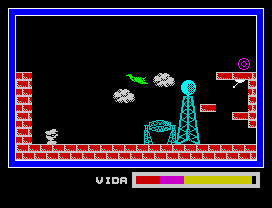
\includegraphics{../images/phantomas-sp1}
\caption{Phantomas (© 1986 Dinamic)}
\label{fig:phantomas}
\end{figure}

\bigskip
Todavía faltaba mucho tiempo para que aprendiera lo que era una interfaz (aún no había aprendido ni tan siquiera a leer) pero ya sabía interpretar algunas letras, curiosamente las que tenían pintadas las teclas OPQA\footnote{En los primeros ordenadores que aparecieron en España en la década de los 80 esta era la combinación de teclas que tenían predefinidos la mayoría de los juegos siendo OP las teclas para moverse de izquierda a derecha y QA para hacerlo de arriba a abajo.}.

\bigskip
Según fui creciendo aprendí a leer y escribir y también a reconocer unos códigos que aparecían al final de las revistas que compraba mi hermano que se llamaban POKES\footnote{Instrucción en lenguaje BASIC que graba un valor en una determinada dirección de memoria.}, estos códigos hacían que, introduciéndolos a la hora de cargar el juego, pudiera tener vidas infinitas, la habilidad de atravesar paredes o la capacidad de ser invisible a los enemigos. Estos trucos permitían a un niño torpe a los mandos, como lo era yo, el poder terminar los dificilísimos juegos de la época.

\bigskip
Pasaron algunos años y ya en el colegio muchos amigos tenían consolas de videojuegos en las que metías un cartucho e instantáneamente estabas jugando a juegos increíbles con una paleta de colores que raro era que no provocara ataques epilépticos. Mientras mis amigos solo tenían que introducir el cartucho y empezar a jugar yo tenía que esperar 5 interminables minutos mientras escuchaba sonidos estridentes y cruzar los dedos por que no apareciera el fastidioso TAPE ERROR que se podía intentar solucionar girando un tornillo llamado ``azimut'' con un destornillador que curiosamente aún poseo.

\bigskip
Y de esta manera, sin siquiera saberlo, tuve mis primeros contactos con el auto-aprendizaje, yo girando un tornillo sin saber a ciencia cierta el por qué y mis amigos el mayor problema que tenían era que a veces tenían que dar un soplido fuerte a la ranura del cartucho.

\bigskip
Mucho mas tarde entró en mi casa un flamante Pentium 166 MMX con Windows 95 OSR2 cuyo entorno tenía ventanas y era bastante intuitivo, podía escribir documentos con formato y el primo de un conocido tenía un programa te marcaba en rojo los errores ortográficos de los trabajos del colegio. De hecho ese mismo señor tenía un CD llamado Encarta donde había toda una enciclopedia metida dentro, solo tenías que escribir una palabra y al momento aparecía su definición con fotografías y todo. Ya no era necesario esperar al día siguiente para poder ojear la enciclopedia del colegio, podía obtener toda la información que necesitara mientras me quemaba las retinas con aquellos monitores de rayos de tubos catódicos.

\bigskip
Estábamos ya a mediados de 1996 y se empezaba a hablar de Internet, era como aquella Encarta pero sin CD, el futuro nuevamente había llegado y todo el dinero invertido en una grabadora de CD se iba al garete, junto con las horas mantenidas cruzando los dedos y sin tocar el ordenador para que fallara la grabación, todo estaba en Internet, y si no estaba ahí poco tardaría en estarlo.

\bigskip
Así que cogí los ahorros de mi paga semanal y me compré un módem para puerto serie de 33.000 Baudios de segunda mano. Conecté el módem metí uno de los múltiples de CDs de conexión a Internet que regalaban por aquel entonces con las revistas, le di a conectar y ahí estaban de nuevo las largas esperas escuchando ruidos estridentes igual que unos años antes.

\bigskip
A base de curiosear como buen aspirante a ingeniero vi escondido en las opciones una casilla que decía ``Silenciar altavoz'', ¿como podía ser que millones de personas estuvieran soportando esos ruidos estridente para conectarse por no saber marcar una casilla? Algo raro pasaba ya que la opción estaba ahí pero nadie la pulsaba.

\bigskip
Pasaron los años, los sistemas se fueron haciendo mas complejos y me di cuenta que según más opciones tenían los dispositivos más perezosos se volvían los usuarios. Mi vecino sin ir más lejos por no configurar su televisor tenía TVE2 en el canal 4 de su televisor ¿era yo el único que encontraba eso chirriante? Quizá no, pero como he ido descubriendo hay diferentes tipos de personas, están los que pueden pasar meses alumbrando el pasillo con el teléfono móvil y los que crean un tutorial en YouTube para enseñar a cambiar una bombilla.

\bigskip
Y ese es el deber que tenemos como futuros profesores, ser capaz de transmitir ese conocimiento e intentar que nuestros alumnos no pasen meses a oscuras, que aprendan a silenciar el volumen del altavoz del módem y en el mejor de los casos que sepamos despertar en ellos la curiosidad para que sean ellos mismos los que auto-aprendan y descubran todas esas cosas futuras que aun siendo profesores tenemos por aprender.

\section{Motivación}

Como ya sabemos Internet ha tenido un carácter académico desde prácticamente su nacimiento y por ello las mayores innovaciones y casi todo su enfoque ha salido de estos ámbitos previos a la democratización de la red y el acceso global a Internet. Es impensable concebir hoy día la enseñanza sin hacer uso de Internet y puede que en un futuro no muy lejano la totalidad de la enseñanza se imparta a través de la red.

\bigskip
La labor de un profesor no tiene un horario establecido de 8.00 a 15.00 horas, nuestra labor seguramente será 24/7 los 365 días del año y por eso tenemos que apoyarnos en herramientas que hagan nuestra vida más fácil a la vez que permiten el crecimiento exponencial de la educación.

\bigskip
Personalmente conozco profesores que han coqueteado con sistemas de mensajería instantánea (Telegram) para comunicarse con sus alumnos, dando un servicio mucho mas eficiente y rápido que las clásica tutorías.

Aplicando esa máxima de atender de una manera mas eficaz a nuestros alumnos sin que requiera una inversión adicional de nuestro tiempo...



\section{Definición del problema}


Este proyecto intentará resolver los siguientes problemas:

\begin{itemize}
  \item Evitar la tediosa tarea de la corrección de ejercicios.
  \item Motivar la enseñanza y aprendizaje de la programación a través de ejemplos.
  \item Ver cómo un sistema de control de versiones es una herramienta básica que debería enseñarse a la vez que se enseña programación.
  \item Mejorar la calidad de vida tanto de profesores como de estudiantes
\end{itemize}

\section{Estructura del proyecto}


\bigskip
Antes de pasar a detalles más técnicos, me gustaría detallar el contenido de este proyecto:

\begin{itemize}
  \item En el \textit{capítulo 1} (\textbf{Introducción}) se encuentra un texto descriptivo del proyecto, así como una breve introducción a las tecnologías que se utilizarán.\cite{QueueSystems}
  \item El \textit{capítulo 2} (\textbf{Objetivos}) detalla de forma algo más concreta los objetivos determinados que se quieren cumplir con este proyecto.
  \item En el \textit{capítulo 3} (\textbf{Metodología}) está la planificación y desarrollo de cada uno de los apartados del proyecto.
  \item En el \textit{capítulo 4} (\textbf{Resultados})se detallan todos los resultados obtenidos.
  \item En el \textit{capítulo 5} (\textbf{Conclusiones}) se pueden encontrar las conclusiones finales  así como las recomendaciones para futuros trabajos.

\end{itemize}


\bigskip
Para finalizar se incluye un anexo con el código fuente desarrollado y liberado bajo una licencia libre.


% %
% % Ejemplos de codigo LaTeX para uso futuro
% %

% \begin{figure}[h!]
% \centering
% 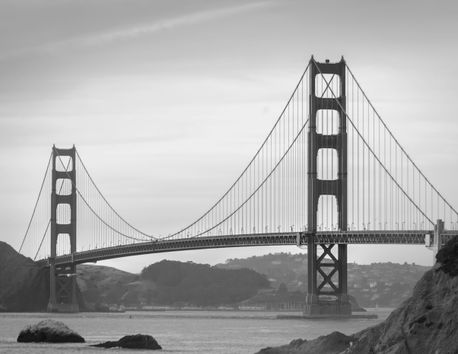
\includegraphics{../screenshots/sample1}
% \caption{Sample Image 1}
% \label{fig:sample1}
% \end{figure}

% Esto es un texto con una nota\footnote{Ejemplo de nota al pie} al pie.

% Y esto es una ``Frase de alguien''\cite{stevekrug}.

% \begin{itemize}
%   \item \textbf{1.} Texto de ejemplo
%   \item \textbf{2.} Texto de ejemplo
%   \item \textbf{3.} Texto de ejemplo
%   \item \textbf{4.} Texto de ejemplo

% \end{itemize}

% \begin{enumerate}
% 	\item Ejemplo 1.
% 	\item Ejemplo 2.
% \end{enumerate}

% \begin{lstlisting}[language=html]
% <!DOCTYPE html>
% <html lang="es-ES">
%   <head>
%     <meta charset="utf-8">
%     <title>Ejemplo de 2 párrafos</title>
%   </head>
%   <body>
%     <p>Esto es un párrafo.</p>
%     <p>Esto es otro párrafo.</p>
%   </body>
% </html>
% \end{lstlisting}

% Puedes verlo en \cite{Patricio2011}. Te recomiendo leer \cite{Patricio2011, Zacarias2009, Alfonso2010b, Alfonso2010a}.
